\Minisec{Sicherheit}
Sicherheitsziele: Vertraulichkeit, Authentizität, Integrität, Anonymität, $\dots$


\Minisec{Betriebsmodi: }
Codebook Mode: Jeder Block einzeln verschlüsselt\\
CBC: Änderung der Nachricht => keine Mustererkennung\\
Counter mode: Simuliert Stromchiffre mit Pseudozufallsgenerator (aus Nonce)\\
\begin{tabular}{cc}
\textbf{Cypher Block Chaining} & \textbf{Counter Mode}\\
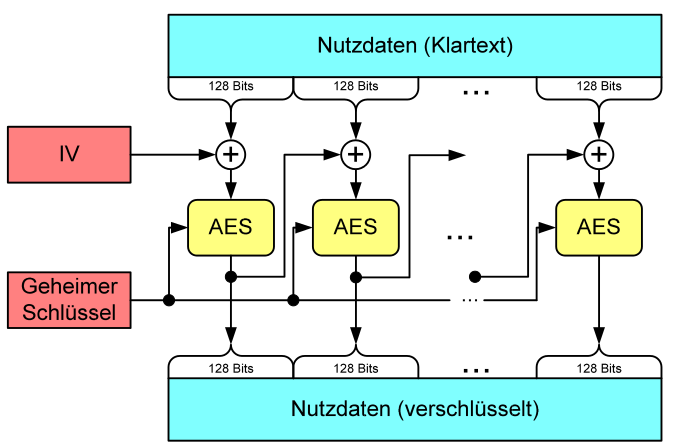
\includegraphics[width=0.25\textwidth]{CBC}   &  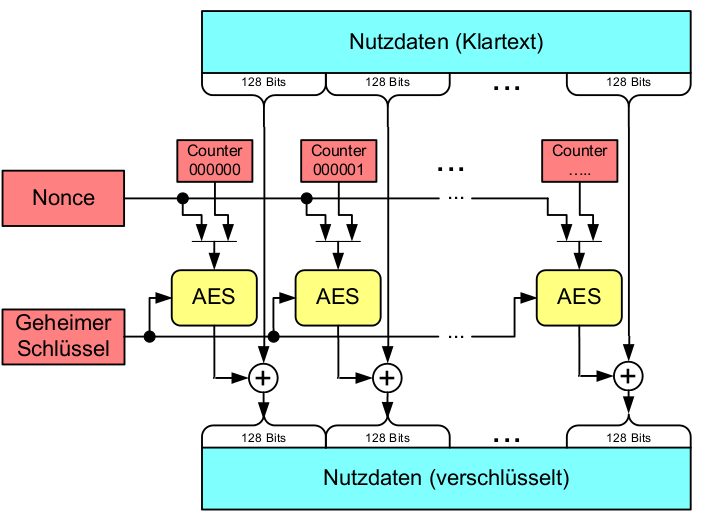
\includegraphics[width=0.25\textwidth]{Counter}\\
\end{tabular}




\Minisec{Rainbow Table: }
\textbf{Erstellen einer Zeile:} beginne bei Startwert, wiederhole Hash- und Reduktionsfunktion bis zum k-ten Hashwert (k=Kettenlänge), speichere Start und Endwert (letzter Hash);\\
\textbf{suchen:} wiederhole Hash und Reduktion bis ein bekannter Endwert, dann gehe vom Startwert mit Hash und Reduktion bis gesuchter Wert erreicht wird\\
\textbf{Salzen:} erzeugen und Speichern von Zufallszahl, hashen von Passwort und Salz
